\documentclass[a4paper,twoside]{article}
\usepackage{graphicx, fullpage, float, verbatim,amsmath, subcaption, listings}

\title{Evolution of CO2e multipliers over time: the case of French Agriculture}
\author{Molly Bazilchuk & Mohamed Badr}
\date{\today}


\begin{document}
\maketitle
\vspace{3cm}
\bibliographystyle{abbrv}

\section{Introduction}

Globally, food production is responsible for around one-quarter of the world's greenhouse gas emissions, while agriculture, forestry and land-use change account for around 18\% \cite{ritchie_roser_2020}. Reducing agricultural emissions will therefore be key in limiting the extent of climate change. In terms of agricultural, France is the largest producer in Europe and is therefore an interest case for study when considering emissions intensity change over time. The French Ministry for Agriculture and Food stated in 2018 their goal to reduce emissions by 50\% by 2050 compared to 1990 levels. Reporting to the EU indicates that emissions from french agriculture have decrease by around 5\% in the period 2005-2019 \cite{euAgricultureEmissions}. However, as is the case with the majority of government pledges, this relates to direct emissions rather than footprint or consumption-based emissions. 

In this work, we perform an input-output analysis of the agricultural products of France. The greenhouse gas multipliers are considered in particular, in order to decouple changes in the production intensity from effects of the final demand. While many IO studies choose to aggregate products in input-output tables to more general categories, we have kept the original agricultural sectors to profit from the detail available in the input-output data. Our research questions were:

\begin{enumerate}
\item To what extent have the multiplier values for the French agricultural sector changed since 1996? 
\item How significant is inflation to understanding this change? 
\item Has the change in multipliers led to a decrease in the total carbon footprint of the 15 agricultural products? 
\end{enumerate}

Previous work has considered either agricultural footprint or evolution in multipliers, but not the two simulatneously. Lee \& Schluter first presented considered multipliers in the context of inflation using input-output, but for an economic rather than an environmentally extended system \cite{Lee1977}. Haggblade et al. looked at agricultural growth multipliers, but once again from an economic perspective \cite{haggblade1991modeling}. Liu et al. looked at the change of pollutants and carbon emissions multipliers in China in the period 2007 - 2012, considering overall changes in the different sectors of the economy \cite{Liu2017}. Camanzi et al. consider agriculture in the EU in particular, and maintained product category resolution in their analysis, but considered the total emissions only rather than the multipliers \cite{Camanzi2017}. Schneider et al. considered the energy intensity of global agriculture and how it has evolved since the 1960's, but the analysis is based on broader economic data rather than input-output tables and so lacks sector evolution \cite{Schneider2009}. Li et. al harness the World Input-Output database to understand the main drivers of CO2 emissions from European Union agriculture by looking at and comparing the agricultural sectors of 18 European economies \cite{Li2016}. In cases like these EXIOBASE stands out with regards to the environmental extensions, as well as sectoral detail. Efforts to look at the footprint of food often use bottom-up/LCA based methods, as was done when the French diet was considered by Barbier et al. \cite{Barbier2019}. There has been limited research done on greenhouse gas multiplier values with regards to specific sectors, and to our best knowledge, our research presents a novel method and findings.

\section{Methods and data}

\subsection{Database}

The analysis was performed using EXIOBASE 3, the multi-regional input-output database with high sectoral resolution (200 products) and emphasis on environmental extensions \cite{Stadler2018}. The scope of our model system was the 15 primary agricultural products. There are also secondary agricultural products (e.g. "dairy products" as opposed to "cattle"), but as our focus was on the production itself we excluded these. Due to computational limitations, we studied every other year starting from the year 1996 and ending at the year 2022. Relevant code can be found in the Appendix.

\subsection{Calculations}

For an input-output system, a multiplier is a quantity that, when multiplied with the final demand, gives the total emissions of a pollutant or other quantity such as energy consumption, labor use, etc. Multipliers $M$ are derived by performing the firm balance for some amount of emissions $F$, where $Z$ is the inter-industry flow matrix describing intermediate demand flowing between industries, and $x$ is the total output vector.

\begin{equation}
F + M Z = M \hat{x}
\end{equation}

We can then rearrange and express as a function of the Leontief inverse $L$ for a system.

\begin{equation}
M = F \hat{x}^{-1} (I - A)^{-1} = f \hat{x} L
\end{equation}

Finally, the total consumption-based footprint can be found using the multipliers by performing:

\begin{equation}
D_{cba} = M Y
\end{equation}

Where $Y$ is the final demand for the products of each sector.

These calculations were performed using the Pymrio Python package \cite{stadler2021}.

\subsection{Impacts}

Impacts were aggregated into GHG emissions “(GWP100) | Problem oriented approach: baseline (CML, 2001) | GWP100 (IPCC, 2007)”. This is done through characterization, which allows us to gain a broader perspective of all the GHG related impacts per product. After a primary analysis we then normalise all the multiplier values on the base year of 1996. This allows the research to better understand the evolution of multiplier values within a given time frame.

\subsection{Inflation}

To adjust for inflation, we use the Food and Agriculture Organisation of the United Nations (FAOSTAT) data on inflation in the French agricultural sector in the relevant time frame. Given the absence of product specific inflation statistics, this was the most relevant inflation data available. We normalise all prices on the base year 2015 as per FAOSTAT. Given that FAOSTAT only provides inflation figures from the year 2000 we used the inflation rate for the year 2000 for the years 1996 and 1998. More so, the inflation rate for the year 2022 has not been released yet (for the relevant sectors), we therefore use the inflation rate of the previous year (2021).

\section{Results}

Fig. \ref{fig:rawmultipliers} shows the evolution of the agricultural multipliers from the year 1996 - 2022 as obtained directly from the Pymrio calculation. We can see that animal production sectors such as cattle, animal products, raw milk and meat animals nec have by far with largest multipliers per euro sold. This again is for the production sectors, whereas EXIOBASE incorporates other product sectors for the final products as sold to consumers.

Based on the raw multipliers, it would appear that the trend is a decrease in multipliers over the time period considered. However, as we will see in the next figure, this is misleading.

\begin{figure}[H]
\centering
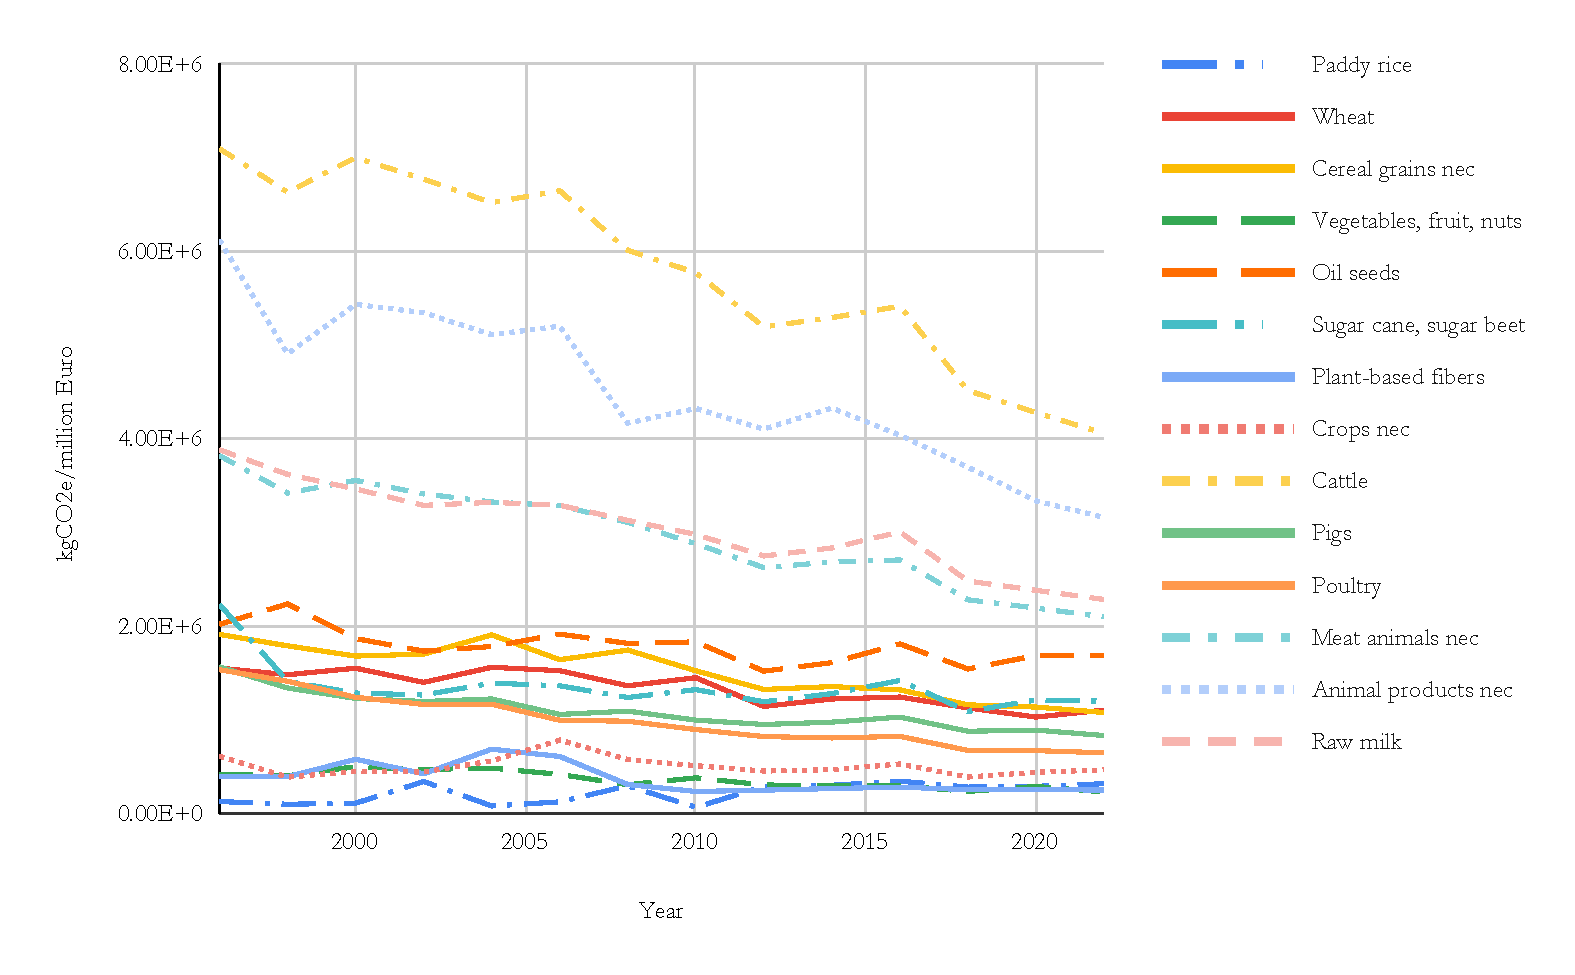
\includegraphics[width=0.9\textwidth]{raw_multipliers}
\caption{The multipliers per sector for French agriculture 1996 - 2022.}\label{fig:rawmultipliers} 
\end{figure}

Since multipliers are expressed in terms of currency, changes over time cannot be properly considered without taking into account the effects of inflation. The multipliers were therefore adjusted using the consumer price indices from FAOSTAT. The consumer price indices are given with a base year of 2015, such that the multipliers for earlier years are general lower that in Fig. \ref{fig:rawmultipliers} and later years increase.

Fig. \ref{fig:adjustedmultipliers} shows the inflation-adjusted multipliers for the agricultural sectors. The downward trend is now far less prominent. 

\begin{figure}[H]
\centering
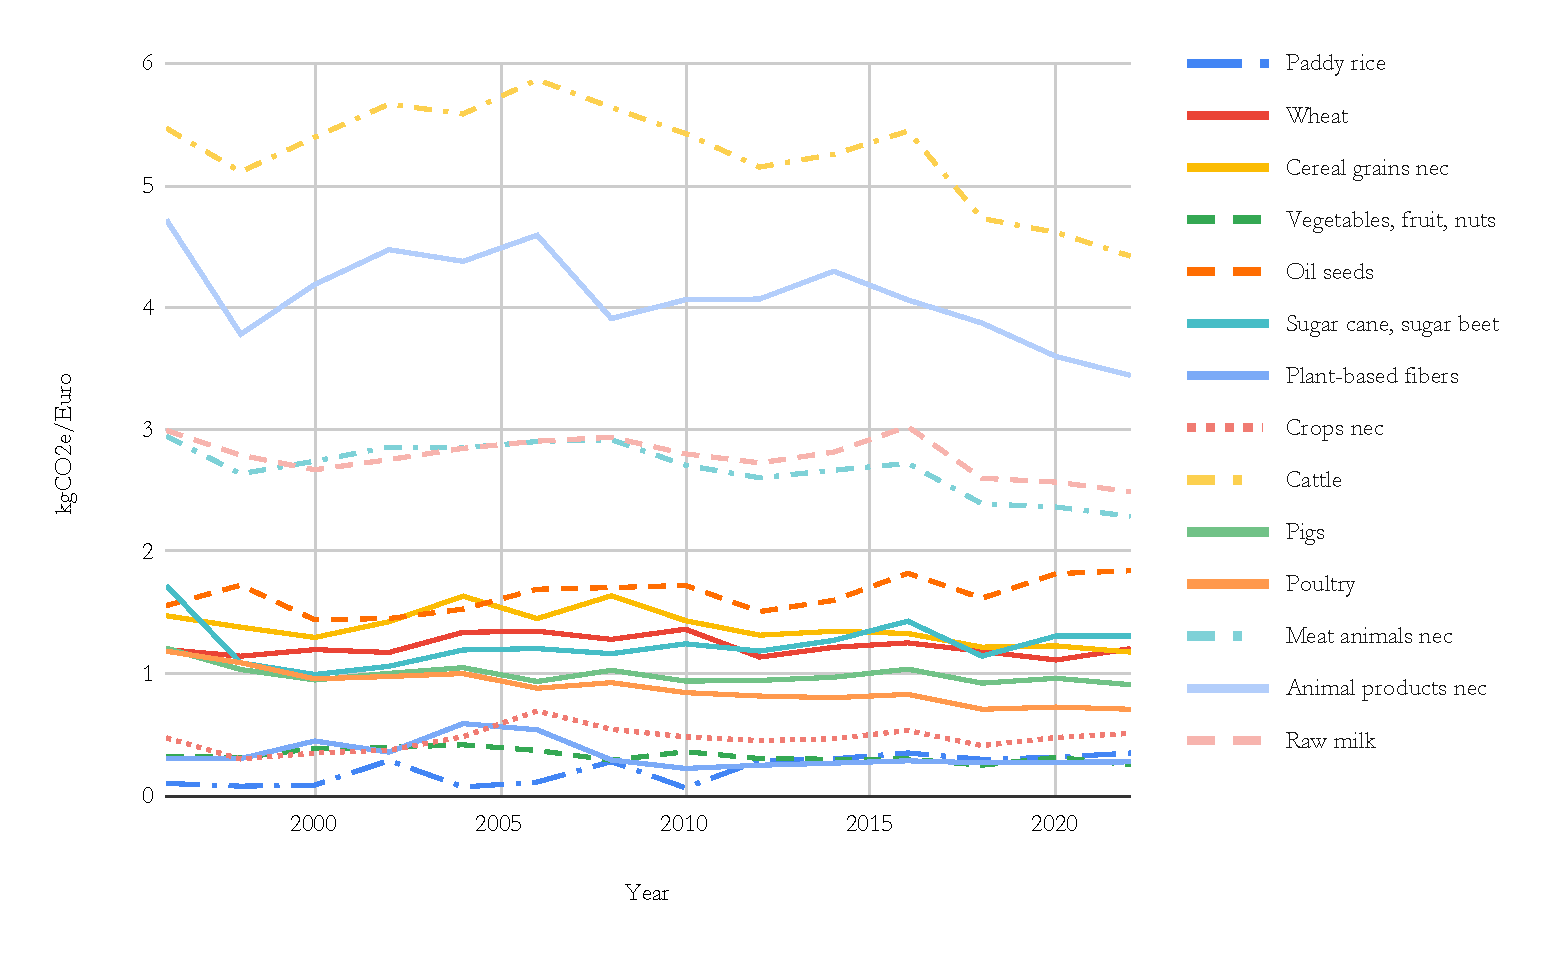
\includegraphics[width=0.9\textwidth]{inflated_adjusted}
\caption{The inflation-adjusted multipliers per sector for French agriculture 1996 - 2022}\label{fig:adjustedmultipliers} 
\end{figure}

In order to determine the trend in the evolution of the multipliers, the data was normalized relative to the starting year (1996) and the data for each sector was fit to a line using linear regression. The slope of the line then gives us the average percent-wise change of the multipliers per year. Fig. \ref{fig:slope} shows the slopes of the normalized multipliers, ordered from smallest to largest. 

\begin{figure}[H]
\centering
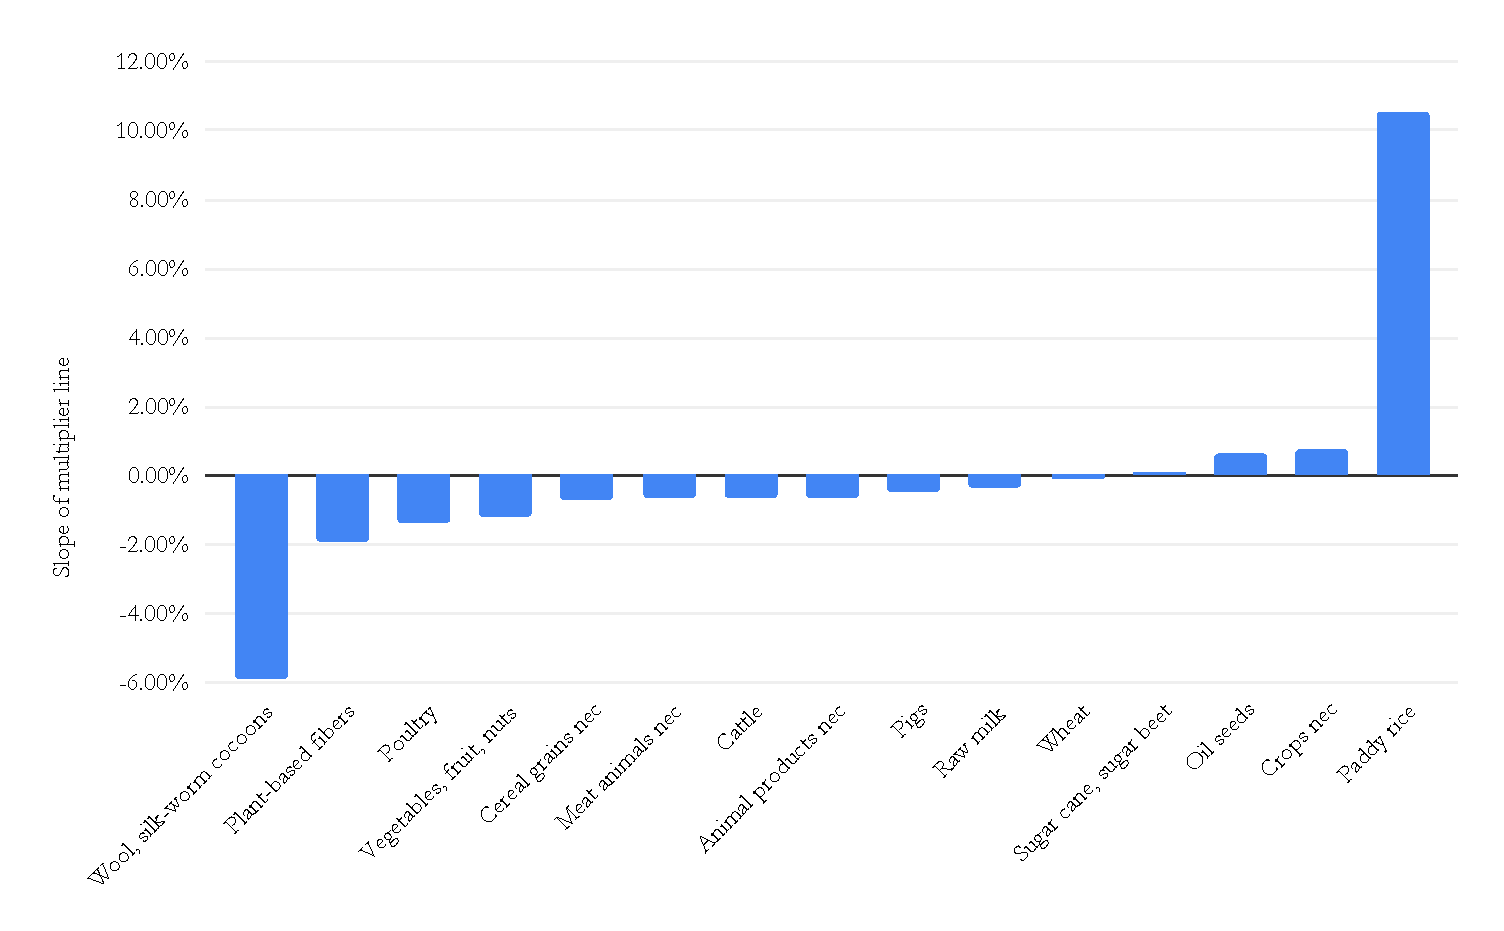
\includegraphics[width=0.9\textwidth]{slope}
\caption{The slope of the normalized multiplier line for each sector for the period 1996 - 2022}\label{fig:slope} 
\end{figure}

The average slope was -0.12\% per year, indicating that the multipliers are in fact trending very slightly downward. From Fig. \ref{fig:slope} it can be clearly seen that most slopes were less than -2\% per year. Outliers are the sectors "wool, silk-worm cocoons" and paddy rice. Wool trends strong negative, but this is mostly due to the erratic behavior of this particular sector, which exhibited a large spike around 2008 before decrease towards 2022 and landed at essentially the same value as 1996. Paddy rice exhibits a strong increase of over 10\%, but has the lowest multiplier in terms of absolute value to begin with. The multipliers with the largest absolute value (cattle, raw milk, etc) exhibit the least amount of change.

In order to put the findings in context, we additionally calculated the total agricultural footprint by summing the total impacts for each of the sectors considered. Fig. \ref{fig:totalfootprint} shows the total footprint for agricultural sectors of France during the time periode considered. Despite some oscillations, the footprint increases slightly over the period considered.

\begin{figure}[H]
\centering
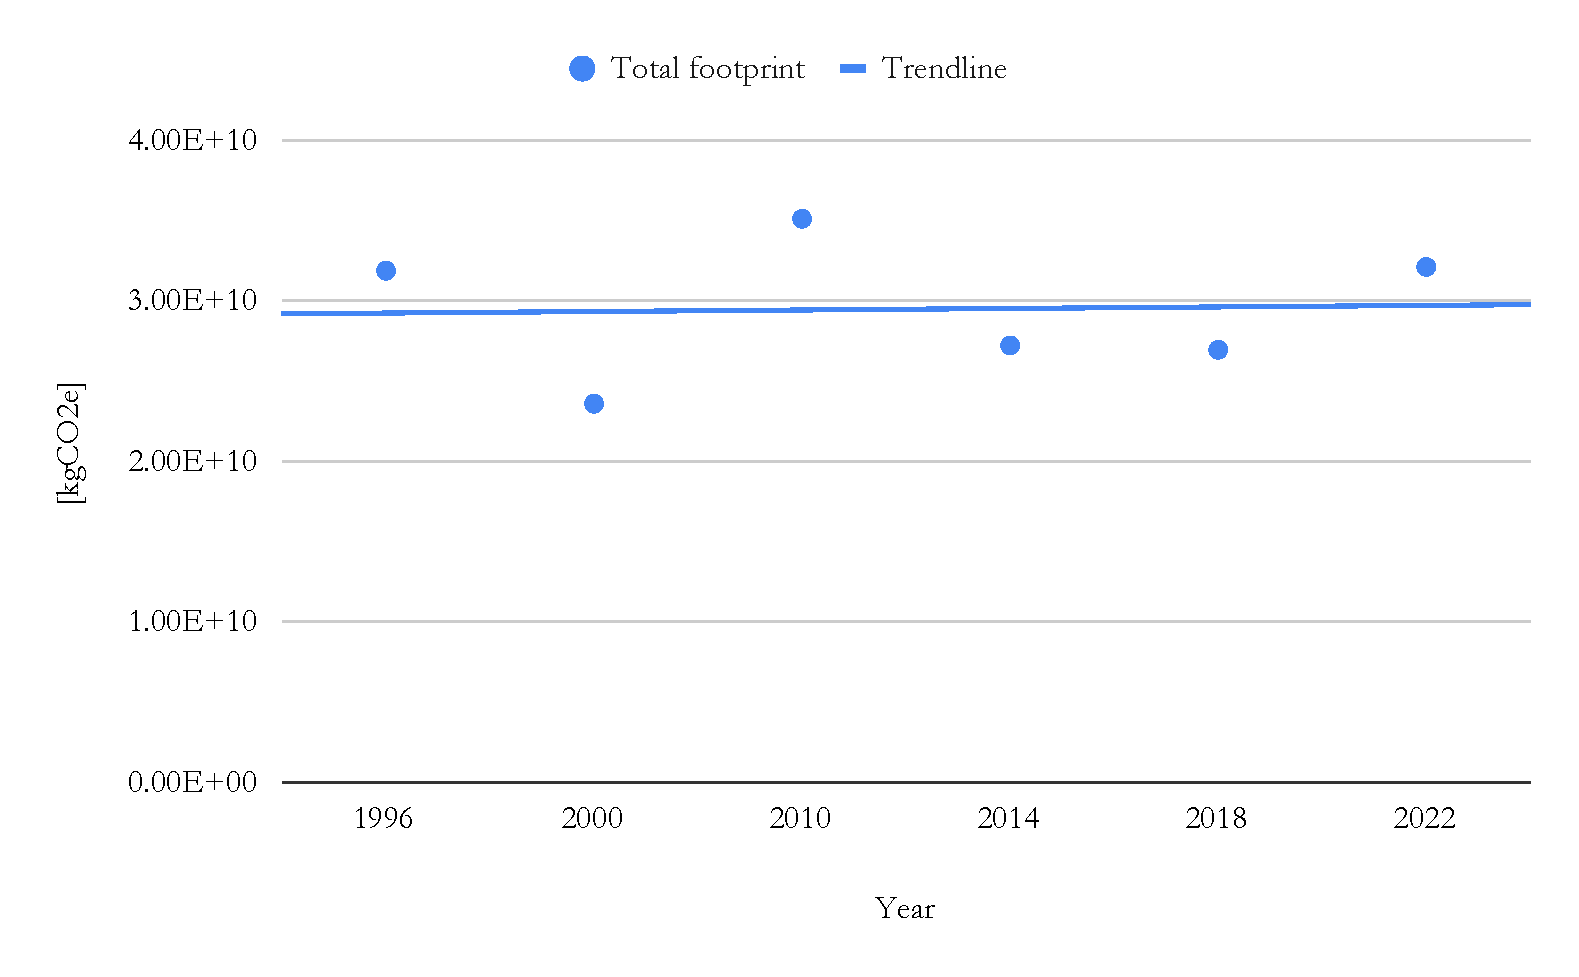
\includegraphics[width=0.9\textwidth]{totalfootprint}
\caption{The slope of the normalized multiplier line for each sector for the period 1996 - 2022}\label{fig:totalfootprint} 
\end{figure}

\section{Discussion and conclusion}

We have considered the evolution of French agricultural multipliers over the time period 1996 - 2022, using the high sectoral resolution of EXIOBASE to visualize changes in individual sectors. As expected, the largest multipliers where those associated with products of animal husbandry. With a few exceptions, the multipliers remained relatively constant over the time period considered, generally changing less that 2\% per year. The overall trend was a weak decrease in multiplier, which could indicate that some progress is being made in production efficiency. Interestingly, the work of Schneider et al. indicated a stagnation in the relative energy efficiency of agricultural production since the 1990's \cite{Schneider2009}. The trend of the multipliers is in line with this finding, as we don't see indications of significant technological progress.

The calculated multipliers were adjusted to inflation rates using consumer price indexes from FAOSTAT. Inflation is significant in understanding the change in multipliers, as the trend in all sectors shifts from decreasing to almost flat when they are incorporated. However, it should be considered that applying the FAOSTAT index is a simplification, as inflation in certain sectors of agriculture might be larger than others. Furthermore, the inflation indices are for end consumer prices whereas we are considering primary agricultural products. This uncertainty along with the weak trend of multiplier changes means that the multipliers could be considered to be essentially stable over the time period considered. 

France has reported a decrease in agriculture emissions, whereas we find that the agricultural \emph{footprint} is actually slightly increasing. This could indicate a shift from direct to embodied emissions, although further work is needed to examine the decoupling of emissions and footprint for French agriculture. Overall, we did not observe significant improvements in the footprint of the agricultural sector in France.


\bibliography{IOreport}

\appendix

\section{Python code}

\begin{lstlisting}

# Load Libraries
import pymrio
import numpy as np
import pandas as pd

# Define Inputs
Country = 'FR'
charact_table = pd.read_csv('public_char_factors.csv',  sep='\t')
ghg = 'GHG emissions (GWP100) | Problem oriented approach: baseline (CML, 2001) | 
GWP100 (IPCC, 2007)'

years = [str(year) for year in [*range(1996, 2024, 2)]]

# Next we iterate over the year range
for year in years:
  currentpath = 'IOT_'+year+'_pxp.zip'
  # Load data
  print('Loading data for ', year)
  current_exio = pymrio.parse_exiobase3(path=currentpath)
  # Calculate system
  print('Calculating data for ', year)
  current_exio.calc_all()
  # Characterize system
  print('Characterizing data for ', year)
  current_multiplier = current_exio.impacts.M[Country].loc[[ghg]].iloc[:, 0:15]
  # Store relevant multipliers
  current_multiplier.to_excel('multipliers'+year+'.xlsx')
  # Print total agricultural footprint
  current_footprint = current_exio.impacts.D_cba[Country].iloc[:,0:15].loc[ghg].sum()
  print('Total agricultural footprint for ', year, ' was ', current_footprint, 
  ' kgCO2e')
  print('Calculation for year ', year, ' complete')
  
\end{lstlisting}

\end{document}